
\section{Fonctions numérique de la variable réelle : Généralités et définitions}

\subsection{Fonction}

\begin{tabular}{lll}
Soit & $f:$ & $ \R \rightarrow \R$ \\
& & $x\mapsto \underbrace{f(x)}_{\textrm{image de} x}$ \\
\end{tabular}

$f$ est une fonction numérique de la variable réelle si et seulement si :

\textbf{Tout élément de $\mathbf{\R}$ a au plus une image dans $\mathbf{\R}$.} \\

\textbf{Remarques}

\begin{itemize}


\item[*]Vocabulaire : "Au plus une" veut dire, soit une, soit aucune. \\ 

\item[*] $f$ est une fonction et $f(x)$ un nombre réel.
\end{itemize}
\subsection{Ensemble de définition d'une fonction}

\begin{tabular}{lll}

Soit & $f:$& $ \R \rightarrow \R$ \\
& & $x\mapsto f(x)$ \\
\end{tabular}

\textbf{L'ensemble de définition de f, noté $ \mathbf{D_f} $, est l'ensemble de élément de $\mathbf{\R}$\\qui ont une image dans $\mathbf{\R}$}


\begin{minipage}{5cm}
\begin{tikzpicture}[scale=.8]

\tkzDefPoint [label=left:$a$](0,1.5){a}
\tkzDrawPoint[size=10,color=black](a)
\tkzDefPoint [label=left:$b$](0,1){b}
\tkzDrawPoint[size=10,color=black](b)
\tkzDefPoint [label=left:$c$](0,.5){c}
\tkzDrawPoint[size=10,color=black](c)
\tkzDefPoint [label=left:$d$](0,0){d}
\tkzDrawPoint[size=10,color=black](d)
\tkzDefPoint [label=right:$\Delta$](3,1.5){de}
\tkzDrawPoint[size=10,color=black](de)
\tkzDefPoint [label=right:$\bigstar$](3,1){st}
\tkzDrawPoint[size=10,color=black](st)
\tkzDefPoint [label=right:$\bigcirc$](3,.5){nada}
\tkzDrawPoint[size=10,color=black](nada)



\node [draw,ellipse,minimum height=3cm,minimum width=1.5cm, fit={(a) (b) (c) (d) }] {};
\node [draw,ellipse,minimum height=3cm,minimum width=1cm,fit={(de) (st) (nada) }] {};

\draw  [bend left=20,-latex](a) to (de) ; 
\draw  [bend right=20,-latex](b) to (de) ; 
\draw  [bend right=20,-latex](c) to (st) ; 
\end{tikzpicture}
\end{minipage}
\begin{minipage}{3cm}

$f(a) = \Delta$

$f(b) = \Delta$

$f(c) = \bigstar $ \\

$ D_f = \lb a, b, c \rb $

$D_f = E \setminus\lb d \rb $

\end{minipage}\\


\subsubsection{Exercice \no 1}

\begin{tabular}{llll}
Soit & $f:$& $ \R \rightarrow \R$ & \\
& & $x\mapsto f(x)$ & $=\dfrac{x-4}{x-2}$ \\
\end{tabular}\\

Il ne faut pas que $x-2=0$, donc que $x=2$.

$D_f = \R \setminus \lb 2 \rb = \left]-\infty,2\right[\cup\left]2, +\infty\right[$

\subsubsection{Exercice \no 2}

\begin{tabular}{llll}

Soit & $f:$& $ \R \rightarrow \R$ & \\
& & $x\mapsto f(x)$ & $=\sqrt{x-2}$ \\
\end{tabular}\\

Il faut que $x-2 \geqslant 0$, donc que $x \geqslant 2 $

$D_f = \left[2, +\infty\right[ $

\newpage

\subsubsection{Exercice \no 3}

\begin{tabular}{llll}

Soit & $f:$& $ \R \rightarrow \R$ & \\
& & $x\mapsto f(x)$ & $=\dfrac{x^2 + 4}{x^2 - 4}$ \\
\end{tabular}\\

Il ne faut pas que $x^2 - 4 = 0$, donc que $\left(x+2\right)\left(x-2\right) = 0 $

\begin{tabular}{lll}
$x+2=0$ & ou & $x-2 = 0 $ \\
$x = -2 $ & ou & $x=2$ \\
\end{tabular}

$ D_f = \R \setminus\lb -2,2\rb = \left]-\infty, -2\right[\cup \left]-2,2\right[\cup\left]2, +\infty\right[ $

\subsubsection{Exercice \no 4}

\begin{tabular}{llll}

Soit & $f:$& $ \R \rightarrow \R$ & \\
& & $x\mapsto f(x)$ & $=\sqrt{x^2 - 4}$ \\
\end{tabular}

Il faut que $x^2 - 4 \geqslant 0 $, donc que $\left(x+2\right)\left(x-2\right) \geqslant 0$

\begin{tikzpicture}
\tkzTabInit[lgt=3,espcl=2]
{ $x$  /1,
$x+2$ /1,
$x-2$   /1,
$\left(x+2\right)\left(x-2\right)$ /1}
{$ - \infty $ , $-2 $ , $2 $ , $ + \infty $}
\tkzTabLine{ , - , z , +, t  ,+ }
\tkzTabLine{ , - , t , - , z , + }
\tkzTabLine{ , + , z , - , z , + }
\draw[decoration={brace, mirror, raise=0.2cm}, decorate, line width=2pt,black] (T14) -- (N24) ;
\draw[decoration={brace, mirror, raise=0.2cm}, decorate, line width=2pt,black] (N34) -- (T24) ;
\end{tikzpicture}

$D_f = \left]-\infty,-2\right[\cup\left[2,+\infty\right[ $

\subsubsection{Exercice \no 5}

\begin{tabular}{llll}

Soit & $f:$& $ \R \rightarrow \R$ & \\
& & $x\mapsto f(x)$ & $=\dfrac{x^2 - 4}{x^2 + 4}$ \\
\end{tabular}\\

Il ne faut pas que $x^2 + 4 = 0$, donc $x^2 = -4$.

Ceci est impossible, donc $D_f = \R$.

\textbf{Remarque}

Il s'agit du problème de la continuité.

\subsubsection{Exercice \no 6}

\begin{tabular}{llll}

Soit & $f:$& $ \R \rightarrow \R$ & \\
& & $x\mapsto f(x)$ & $=\sqrt{x^2 + 4}$ \\
\end{tabular}

Il faut que $x^2+4 \geqslant 0$, donc $x^2 \geqslant -4$

Ceci est toujours vrai, donc $D_f = \R$.

\subsection{Représentation graphique d'une fonction}

\begin{tabular}{lll}

Soit & $f:$& $ \R \rightarrow \R$ \\
& & $x\mapsto f(x)$ \\
\end{tabular}\\

Soit $\left(0, \overrightarrow{i}, \overrightarrow{j}\right)$ un repère.

La représentation graphique de $f$, notée $C_f$, est l'ensemble des points $M\left(x,y\right)$ avec $x\in D_f$ et $y = f(x)$.

\newpage

\vspace*{-2cm}
\textbf{I}\\

\centerline{
\begin{minipage}{.45\textwidth}
\shorthandoff{:}
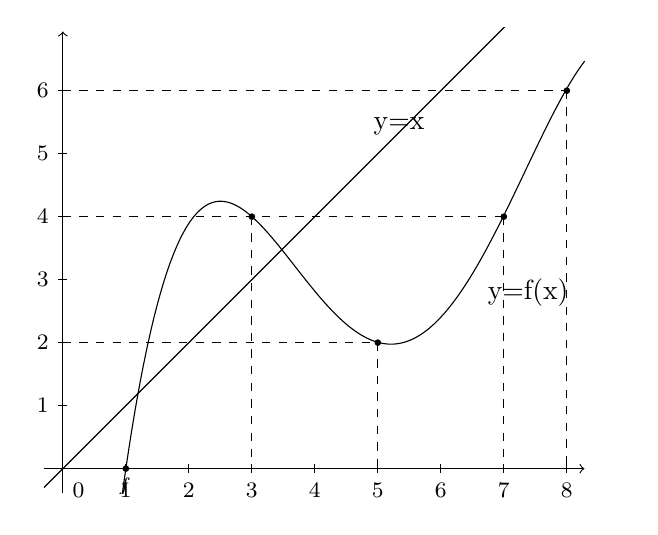
\begin{tikzpicture}[scale=0.8]
\draw[->,color=black] (-0.3,0) -- (8.28,0);
\foreach \x in {,1,2,3,4,5,6,7,8}
\draw[shift={(\x,0)},color=black] (0pt,2pt) -- (0pt,-2pt) node[below] {\footnotesize $\x$};
\draw[->,color=black] (0,-0.38) -- (0,6.94);
\foreach \y in {,1,2,3,4,5,6}
\draw[shift={(0,\y)},color=black] (2pt,0pt) -- (-2pt,0pt) node[left] {\footnotesize $\y$};
\draw[color=black] (0pt,-10pt) node[right] {\footnotesize $0$};
\clip(-0.3,-0.4) rectangle (9,7);
\draw[smooth,samples=100,domain=-0.301:8.284] plot(\x,{
-(29/840)*(\x)^4 
+(213/280)*(\x)^3 
-(4699/840)*(\x)^2 
+(4443/280)*\x 
-11});
\draw [dashed] (3,4)-- (3,0);
\draw [dashed] (0,4)-- (7,4);
\draw [dashed] (7,4)-- (7,0);
\draw [dashed] (0,2)-- (5,2);
\draw [dashed] (5,2)-- (5,0);
\draw [dashed] (0,6)-- (8,6);
\draw [dashed] (8,6)-- (8,0);
\draw[smooth,samples=100,domain=-0.301:8.284] plot(\x,{(\x)});
\draw (6.59,3.17) node[anchor=north west] {y=f(x)};
\draw (4.78,5.72) node[anchor=north west] {y=x};
\begin{scriptsize}
\fill (1,0) circle (1.5pt);
\fill (3,4) circle (1.5pt);
\fill (5,2) circle (1.5pt);
\fill (7,4) circle (1.5pt);
\draw(0.98,-0.29) node {$f$};
\fill (8,6) circle (1.5pt);
\end{scriptsize}
\end{tikzpicture}
\shorthandon{:}
\end{minipage} \hspace*{1cm}
\begin{minipage}{.45\textwidth}
On a représenté ci-contre : \\
\begin{itemize}
\item[*] La droite d'équation $y=x$ ; 
\item[*] La courbe représentative d'une fonction $f$ définie sur l'intervalle $[1;8]$. 
\end{itemize}
Les question posées seront résolues par {\bf lecture graphique}. 
\end{minipage}}
\vspace{.5cm}
Répondre par vrai ou faux aux questions suivantes : 

\vspace{.1cm}

\begin{tabular}{|l|c|l}
\multicolumn{2}{r}{vrai ou faux} & \\
\cline{1-2}
$1$ a pour image $0$ par la fonction $f$ & \textcolor{blue} {\it \Large V } & \\
\cline{1-2}
$0$ a pour image $1$ par la fonction $f$ & \textcolor{blue} {\it \Large F } & \\
\cline{1-2}
$5$ est un antécédent de $2$ par la fonction $f$ & \textcolor{blue} {\it \Large V } & \\
\cline{1-2}
$4$ a deux  antécédents  par la fonction $f$ : $3$ et $7$ &  \textcolor{blue} {\it \Large F}& \\
\cline{1-2}
\textcolor{blue} {\it Combien 3 a-t-il d'antécédents ? }& \textcolor{blue} {\it \Large 3 }&\\
\cline{1-2}
& \\
\cline{1-2}
$f(3) \leqslant f(5) $ & \textcolor{blue} {\it \Large F } &\\
\cline{1-2}
$f$ est croissante sur l'intervalle $[1 ; 8]$ & \textcolor{blue} {\it \Large V } & pas strictement\\
\cline{1-2}
& \\
\cline{1-2}
& \\
\cline{1-2}
L'équation $f(x) = x $ a au moins une solution dans l'intervalle $[1 ; 8]$ &  \textcolor{blue} {\it \Large V } &\\
\cline{1-2}
Si $x$ appartient à l'intervalle $[3 ; 5]$ alors $f(x) \leqslant x $ & \textcolor{blue} {\it \Large F } &\\
\cline{1-2}
\end{tabular}

\medskip 

\textbf{II}\\

On considère la fonction $f$ définie sur l'intervalle $[-7 ; 4]$ par sa représentation graphique $\mathcal{C}$ et la fonction $g$ dont la représentation graphique est la droite $d$.
 
\centerline{
\begin{minipage}{.6\textwidth}
\textbf{Répondre aux questions suivantes par lecture graphique}
\begin{enumerate}
\item  \begin{enumerate}
        \item Quelles sont les images par $f$ des réels $-3$ et $0$ ? 
        \item  Quels sont les antécédents éventuels de $4$ par $f$ ?  
       \end{enumerate}
\item Résoudre graphiquement les équations et les inéquations suivantes en justifiant les réponses ; 
        \begin{enumerate}
        \item $f(x)= 5$ 
        \item $f(x)= g(x)$ 
        \item $f(x)\geqslant 4$ 
        \item $f(x) > g(x)$ 
        \end{enumerate}
\item Dresser le tableau de variations de la fonction $f$.
\end{enumerate}
\end{minipage}\hspace*{1cm}
\begin{minipage}{.35\textwidth}
\definecolor{ffqqtt}{rgb}{1,0,0.2}
\definecolor{ttzzqq}{rgb}{0.2,0.6,0}
\definecolor{qqqqff}{rgb}{0,0,1}
\definecolor{xdxdff}{rgb}{0.49,0.49,1}
\definecolor{cqcqcq}{rgb}{0.75,0.75,0.75}
\begin{tikzpicture}[scale=.4,line cap=round,line join=round,>=triangle 45,x=1.0cm,y=1.0cm]
\draw [color=cqcqcq,dotted, xstep=1.0cm,ystep=1.0cm] (-9,-7.66) grid (6,9.19);
\draw[->,color=black] (-9,0) -- (6,0);
\foreach \x in {-8,-6,-4,-2,2,4,6}
\draw[shift={(\x,0)},color=black] (0pt,2pt) -- (0pt,-2pt);
\draw[->,color=black] (0,-7.66) -- (0,9.19);
\foreach \y in {-6,-4,-2,2,4,6,8}
\draw[shift={(0,\y)},color=black] (2pt,0pt) -- (-2pt,0pt);
\clip(-8.5,-4.5) rectangle (5.5,5.5);
\draw[smooth,samples=100,domain=-7.0:-3.0] plot(\x,{0.5*(\x)^2+3*(\x)+0.5});
\draw (-3,-4)-- (-1,2);
\draw[color=ttzzqq, smooth,samples=100,domain=-7.0:-5.0] plot(\x,{0.5*(\x)^2+3*(\x)+0.5});
\draw [color=ttzzqq] (-1,2)-- (2,5);
\draw [color=ttzzqq] (2,5)-- (4,3);
\draw [color=ffqqtt] (1,4)-- (2,5);
\draw [color=ffqqtt] (2,5)-- (3,4);
\draw[smooth,samples=100,domain=-9.0:6.000000000000002] plot(\x,{(\x)/3-1/3});
\draw (-6.57,4.01) node[anchor=north west] {$ \mathcal{C} $};
\draw (-8.08,-2.08) node[anchor=north west] {$$ d $$};
\begin{scriptsize}
\fill [color=xdxdff] (1,0) circle (1.5pt);
\draw[color=xdxdff] (1.11,0.26) node {$I$};
\fill [color=xdxdff] (0,1) circle (1.5pt);
\draw[color=xdxdff] (0.12,1.27) node {$J$};
\fill [color=qqqqff] (-7,4) circle (1.5pt);
\end{scriptsize}
\end{tikzpicture}
\end{minipage} 
}

\newpage


        
\textcolor{blue} 
{
     \begin{enumerate}
     \item \begin{enumerate}
     	   \item $f(-3)=-4 $\\
     	      $f(0) = 3 $
     	   \item Les antécédents de $4$ par $f$ sont $-7$, $1$ et $3$.
           \end{enumerate}
     \item \begin{enumerate}
           \item $f(x) = 5$\\
               $S = \lbrace 2 \rbrace$ 
           \item $f(x) = g(x) $\\ 
               $S = \lbrace -5, -2\rbrace$   
           \item $f(x) \geqslant 4$\\
              $S = \lbrace -7\rbrace \cup \left[ 1,3\right]$                        
           \end{enumerate} 
     \item $S = \left[ -7, -5\right[ \cup \left] -2,4 \right] $\\
     \vspace{1cm}
   \centerline{\begin{variations}
            x   & -7  &    &   -3  &     &  2  &    &  4   \\ 
            \filet
    \m {f(x)}  & \h{4} & \d &  \b {-4} &  \c & \h{5} & \d & \b{3} \\
   \end{variations}}                                        
     \end{enumerate}   
}






